
Steps taken to process an SQL query
\begin{enumerate}
    \item \textbf{Scan}: identify query tokens (key-words, attribute names, relation names)
    \item \textbf{Parser}: checks the syntax using grammar rules
    \item \textbf{Validation}: check that all attributes and relations are valid
    \item Internal representation of the query: \textbf{Query tree} or \textbf{Query graph (Directed acyclic graph)}
    \item \textbf{Query plan} + query \textbf{optimization}
\end{enumerate}

The \textbf{query optimizer} must produce a good execution plan, and the \textbf{code generator} generates the code to execute that plan. The \textbf{runtime database processor} has the task of running the query code to produce a query result. Figure \ref{fig:chap18-0}

\begin{figure}
    \centering
    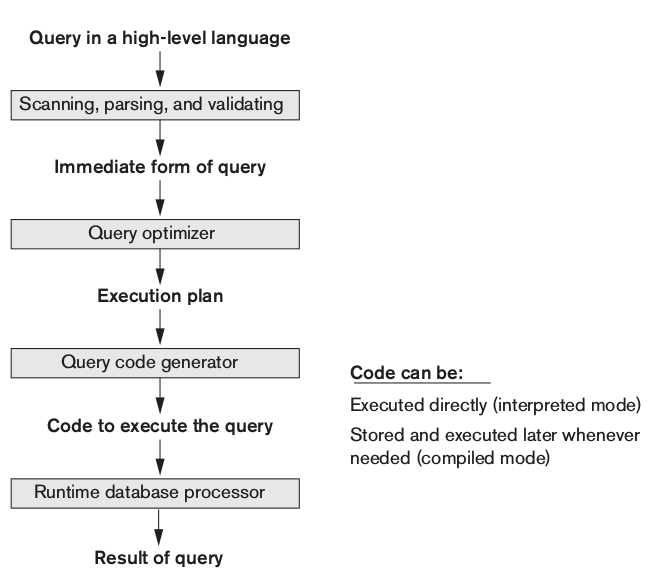
\includegraphics[scale=0.4]{chap18-0}
    \caption{Processing steps of a high-level query}
    \label{fig:chap18-0}
\end{figure}

\section{Translating SQL Queries into Relational
Algebra and Other Operators}

SQL queries are decomposed into \textbf{query blocks} which form the basic units that can be translated into the algebraic operators and optimized. A query block contains a single SELECT-FROM-WHERE expression (and optional GROUP BY and HAVING clauses). Figure \ref{fig:chap18-SQL-Rel}

\begin{figure}
    \centering
    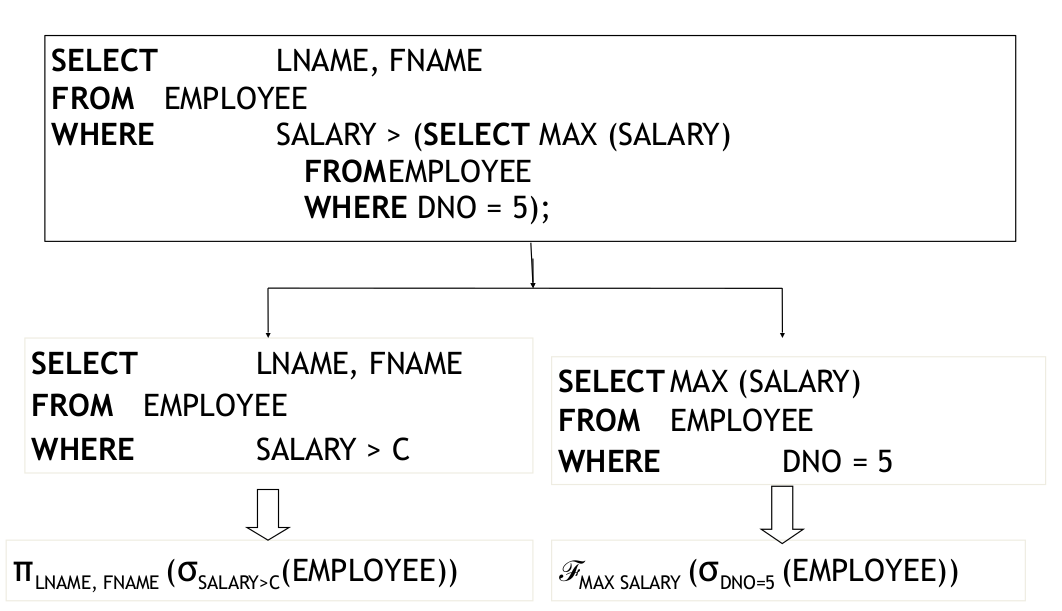
\includegraphics[scale=0.3]{chap18-1}
    \caption{SQL to relational algebra example}
    \label{fig:chap18-SQL-Rel}
\end{figure}

\begin{itemize}
    \item Select operation $\sigma_p(r)$ : Select $p$ from $r$. $p$ is a propositional logic expression
    \item Project operation $\prod_{A_1,...,A_n}(r)$ : projects columns $A_1,...,A_n$ from relation $r$
    \item Union Operation $r U s$: performs the union of relation r and s
    \item Set Difference $r - s$: tuples which are present in one relation but are not in the second relation.
    \item Cartesian Product $r X s$
    \item Rename Operation $\rho_x(E)$: the result of expression $E$ is saved with name of $x$.
\end{itemize}

%\section{Additional Operators Semi-Join and Anti-Join}
%Not important I think.

\section{Algorithms for External Sorting}
\begin{itemize}
    \item Sorting algorithms suitable for large files of records on disk
    \item Do not assume that data fit in main memory
    \item Is used for JOIN, ORDER-BY, etc...
    \item May be avoided by the use of an index.
\end{itemize}

\subsection{Sort-Merge strategy}
\begin{itemize}
    \item Sort small subfiles (runs) of the main file
    \item Merges sorted runs, creating larger sorted subfiles that are merged in turn
\end{itemize} 

\paragraph{Cost}
\begin{itemize}
    \item Sorting phase: Sorting the contents of exactly one disk block. $$nR = \ceil{b/nB}$$
    \item Merging phase: 
    $$dM = \min{(nB-1,nR)}$$
    $$nP= \ceil{\log_{dM}(nR)}$$
    \item Where \begin{itemize}
        \item nR: \# of initial runs
        \item b: \# of file blocks
        \item nB : available buffer space
        \item dM: degree of merging (number of sorted subfiles that can be merged in each merge step). During each merge step, one buffer block is needed to hold one disk block from each of the sorted subfiles being merged, and one additional buffer is needed for containing one disk block of the merge result
        \item nP: \# of passes
    \end{itemize}
\end{itemize}

\section{Algorithms for SELECT Operation}
SELECT = search operation to locate the records in a disk file that satisfy a certain condition. Different search algorithms are possible for selecting records from a file:
\begin{itemize}
    \item Linear search (brute force algorithm)
    \item Binary search (requires ordered file)
    \item Using a primary index or hash key (requires equality comparison on a key)
    \item Using a primary index to retrieve multiple records (requires comparison $>,\geq, <, \leq$ on a key). Use the index to find corresponding equality condition and retrieve all next or previous records in the ordered file.
    \item Using a clustering index to retrieve multiple records (requires equality comparison on a non-key attribute)
    \item Using a secondary ($B^+$-tree) index on an equality comparison. Can be used to retrieve a single record if the indexing field is a key (has unique values) or to retrieve multiple records if the indexing field is not a key.
\end{itemize}

\begin{itemize}
    \item Condition with only one attribute
    \begin{itemize}
        \item If an access path exists, use its corresponding method. Otherwise use brute force.
    \end{itemize}
    \item Condition with more than one attribute
    \begin{itemize}
        \item Query optimization to choose the access path that retrieves the fewest records in the most efficient way 
    \end{itemize}
\end{itemize}

%\section{Estimating the Selectivity of a Condition}
% Skipped

\section{Implementing the JOIN Operation}
Many JOIN are either EQUIJOIN or NATURAL JOIN.
\begin{itemize}
    \item \textbf{two-way join}: join on two files
    \item \textbf{multiway join}: join on more than two files
\end{itemize}
Methods for implementing joins:
\begin{itemize}
    \item \textbf{Nested-loop join} (brute-force).
    \begin{verbatim}
        foreach(t in R)
            foreach(s in S)
                test if t[A]=s[B]
    \end{verbatim}
    
    \item \textbf{Index-based nested-loop join}
    \begin{verbatim}
        foreach(t in R)
            use index or hash to get all matching records s from S such that s[B]=t[A]
    \end{verbatim}
    
    \item \textbf{Sort-merge join} 
    \begin{itemize}
        \item R physically sorted on A
        \item S physically sorted on B
        \item Both files scanned in order of the join attributes
        \item Records of each file are scanned only once (unless both A and B are non-key attributes)
    \end{itemize}
    
    \item \textbf{Hash-join}
    \begin{enumerate}
        \item Records of R are hashed into different buckets (if size of R < size of S, otherwise start with S) (= partitioning).
        \item Records of S are then hashed with the same function, and check if they are present in the bucket (= probing). Only keep the values that were already in the bucket.
    \end{enumerate}
    
\end{itemize}

%\section{How Buffer Space and Choice of Outer-Loop File Affect Performance of Nested-Loop Join}
% Skipped

%\section{How the Join Selection Factor Affects Join Performance}
% Skipped

%\section{General Case for Partition-Hash Join}
% Skipped

% \section{Hybrid Hash-Join}
% Skipped

\section{Algorithms for PROJECT}
A PROJECT operation $\pi_{<attribute list>} (R)$ from relational algebra implies that after projecting R on only the columns in the list of attributes, any duplicates are removed by treating the result strictly as a set of tuples.

\begin{itemize}
    \item If kept attributes include a key of R: extract all tuples from R with only the values for the attributes in attribute list
    \item Otherwise, duplicate tuples must be removed (using sorting or hashing)
\end{itemize}

\section{Algorithms for SET}
\begin{itemize}
    \item INTERSECTION and UNION:
    \begin{itemize}
        \item Sort tuples from both relations on the same attributes
        \item Scan and merge both sorted files concurently
        \item Keep only the tuples that appear in both relations (only keep one for UNION, to have unique tuples)
    \end{itemize}
    \item DIFFERENCE (R-S):
    \begin{itemize}
        \item Keep only those tuples that appear in relation R but not in S
    \end{itemize}
\end{itemize}

% \section{Use of Anti-Join for SET DIFFERENCE (or EXCEPT or MINUS in SQL)}
% Skipped

% \section{Implementing Aggregate Operations and Different Types of JOINs}
% Skipped

% \section{Implementing Different Types of JOINs}
% Skipped

% \section{Combining Operations Using Pipelining}
% Skipped

% \section{Parallel Algorithms for Query Processing}
% Skipped